\label{sec:physical_realism}
Generell ist ein Ziel von physikalischen Simulationen einen realen Sachverhalt möglichst akkurat umzusetzen. Diese Anforderungen sollen für den Verwendungszweck der Simulation als Videospielplattform relativiert werden.\\
In Videospielen dient die Simulation fast ausschließlich der Immersion des Konsumenten, d.h.~der Konsument soll der Illusion von absolutem Realismus erliegen, während dieser aber schwer bis gar nicht umsetzbar sein kann. Es sollte dem Konsumenten möglich sein ein Verständnis für die Vorgänge der Simulation intuitiv entwickeln zu können. Ist dies an Stellen nicht gewährleistet folgt ein Bruch der Illusion, welcher sich negativ auf die Qualität des Produkts auswirkt. In Maßen sind solche Brüche der Illusion nicht kritisch.\\
Videospiele sind generell im Aspekt der Simulationsgenauigkeit im Vergleich mit anderen Applikationen sehr vergebend. Zum Vergleich: Simulationen mit zu niedrigen Fehlertoleranzen in z.B.~der Industrierobotik können zu erheblichem Sach- oder gar Personenschaden führen.\\
Dem Entwickler ist die Aufgabe gestellt, zwischen den Faktoren Performanz, Realismus und Umsetzbarkeit einen Vernünftigen Kompromiss zu finden.\\
Mit diesem kreativen Freiheitsgrad wird allerdings teilweise kritikwürdig umgegangen, indem Missstände in Produkten ignoriert werden und die Frustrationsresistenz des Konsumenten ausgereizt wird, wie dann in Journalismus und Social Media zu lesen ist \cites{unfinished_games0}{unfinished_games1}{unfinished_games2}.\\
Die Unterschiedlichkeit dieser Kompromissfindung kann am Beispiel der Videospiele Minecraft und CSGO betrachtet werden.
\begin{figure*}
\centering
	\begin{subfigure}[t]{0.45\textwidth}
		\centering
		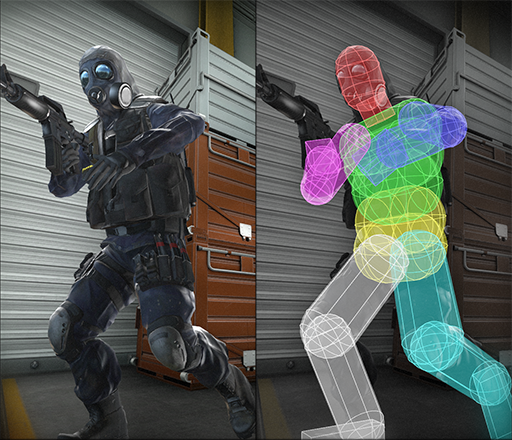
\includegraphics[width=1\textwidth]{./res/csgo_hitbox.png}
		\caption{Hitbox des Spieler-Modells aus dem Videospiel Counter Strike: Global Offensive; sichtbares Modell(links), mit eingeblendeten Hitboxen (rechts)}
%%TODO source for pic
		\label{fig:chitbox}
	\end{subfigure}
~
	\begin{subfigure}[t]{0.2\textwidth}
		\centering
		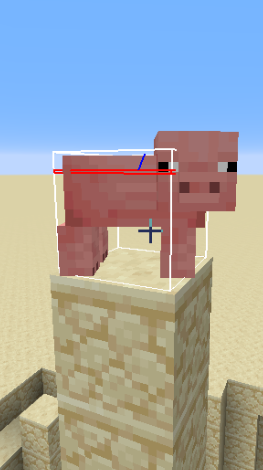
\includegraphics[width=1\textwidth]{./res/pig_hitbox.png}
		\caption{Hitbox eines NPC-Modells (Schwein) aus dem Videospiel Minecraft; Hitbox in weiß}
		\label{fig:mphitbox}
	\end{subfigure}
~
	\begin{subfigure}[t]{0.2\textwidth}
		\centering
		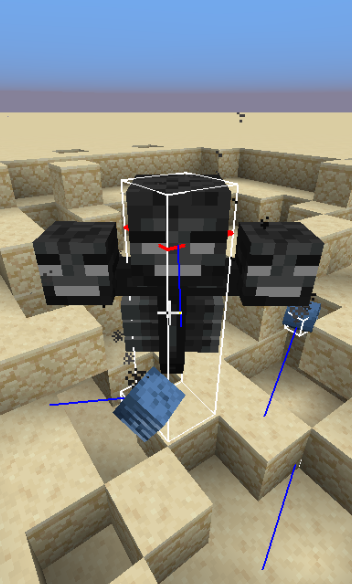
\includegraphics[width=1\textwidth]{./res/wither_hitbox.png}
		\caption{Hitbox eines NPC-Modells (Wither) aus dem Videospiel Minecraft; Hitbox in weiß}
		\label{fig:mwhitbox}
	\end{subfigure}

	\caption{Güten von Hitboxen}
	\label{fig:hitbox}
\end{figure*}

Die Abbildungen~\ref{fig:hitbox} zeigen die Verwendung von Hitboxen \cite{hitbox} in zwei Videospielen, die die kreativen Freiheitsgrade bei der Wahl dieser und ihrer Diskrepanzen verdeutlichen sollen.\\
\ref{fig:chitbox} zeigt das Spielermodell aus dem Spiel Counter-Strike: Global Offensive (CSGO). Die angezeigten Hitboxen sind hier Ellipsoide.
Die Verwendung mehrerer Hitboxen für ein Modell ist ebenfalls zu erkennen.
Einzelne Details des Spielermodells, wie Riemen und Taschen an der Ausrüsung, sind im Spiel nicht essentiell und werden daher auch nicht von den Hitboxen abgebildet.\\
CSGO ist ein hoch kompetitiver E-Sport Shooter, der professionell gespielt wird.
Die Partition der Hitboxen in CSGO ergibt sich direkt aus einer Anforderung der Anwendung, Schusstreffer auf verschiedene Teile des Spielermodells unterschiedlich zu bewerten. Beispielsweise verursacht der Treffer am Kopf am meisten Schaden. Schnelle Reaktion und genaues Zielen sind eine Hauptanforderung an den Spieler. Akkurate und aus der Perspektive des Spielers deterministische Hitboxen sind daher essenziell für das Produkt. In der professionellen Szene geht es dabei um Preisgelder bis in den siebenstelligen Bereich \cite{csgoprice}.\\
Abbildungen~\ref{fig:mphitbox} und~\ref{fig:mwhitbox} zeigen Hitboxen aus dem Spiel Minecraft bei zwei Nicht-Spieler-Charakteren (NPCs). Die hohe Diskrepanz zwischen der Hitbox und dem grafischen Modell ist merklich. Die Minecraft-Hitboxen sind koordinatenachsenparallel, d.h.~Kanten verlaufen immer entlang der Koordinatenachsen der Raumrepräsentation und drehen sich nicht bei der Drehung des Modells mit diesem mit, wodurch die Diskrepanz der Hitbox zum Modell mit dessen Rotation variiert.\\
In Minecraft steckt auch eine erhebliche Summe Geld. Am 15. September 2014 kaufte Microsoft die Entwicklerfirma und die rechte am Spiel für ca. 2,5 Milliarden Dollar \cite{buyminecraft}.\\
Minecraft ist nicht mit Fokus auf schnelle Spieler-gegen-Spieler Szenarien kreiert. Die gesamte Spielwelt ist aus sichtbaren achsenparallel aufgestellten Würfeln aufgebaut, welche durch achsenparallele Hitboxen perfekt abgebildet werden können. Minecraft macht es sich weiter offenbar einfach und verwendet diese an Modellen wieder. Tatsächlich werden künstlich kleinere Hitboxen manchmal sogar eingesetzt um einen Treffer künstlich zu erschweren (vgl. Abbildung \ref{fig:mwhitbox}, bei der die seitlichen Köpfe der Kreatur nicht von der Hitbox eingeschlossen werden).\\
Vielleicht mag eine indirekt proportionale Korrelation zwischen der Diskrepanz bei Hitboxen und Erfolg bestehen, jedoch kann die Kritikalität von Diskrepanz nicht in allen Fällen bestätigt werden.\\

Die Anforderungen in diesem Projekt hinsichtlich physikalischen Realismus werden demnach relativiert. Es bestehen Freiheitsgrade in sowohl der Definition der physikalischen Vorgänge als auch der algorithmischen Umsetzung. 
Videospiele, als Kunstform, können so auch surreale Konzepte umsetzen und Echtzeitanforderungen können leichter eingehalten werden.
